\documentclass[openany]{book}
\usepackage{amsfonts}    % for math fonts
\usepackage{amsmath}     % for advanced math environments

\usepackage{amssymb}     % for math symbols
\usepackage{graphicx}    % for including images

\usepackage{mathpazo}  % Use Palatino as the main font

% Set custom page size and margins using geometry package
\usepackage[paperwidth=6in, paperheight=9in, margin=0.75in]{geometry}

\usepackage{setspace}
\onehalfspacing  % or \doublespacing or \setstretch{1.3}

% Custom chapter titles
\usepackage{titlesec}

\usepackage{xcolor} % Ensure this is loaded
\usepackage{fancyhdr}

\usepackage{makeidx} % Create index
\makeindex

% Adjusting head height for fancyhdr package
\setlength{\headheight}{15pt}

\pagestyle{fancy}
\fancyhf{} % Clear all headers and footers to start fresh

\fancyhead[L]{\textcolor{gray}{\leftmark}}  % Gray color for headers
\fancyfoot[C]{\textcolor{gray}{\thepage}}   % Gray color for page number

% The following line is necessary to remove the default header styling of the 'book' class
\renewcommand{\headrulewidth}{0pt}
\renewcommand{\chaptermark}[1]{\markboth{#1}{}}

% Customizing the chapter title appearance
\titleformat{\chapter}[hang]
  {\normalfont\LARGE\bfseries}{\thechapter\hspace{20pt}}{0pt}{\LARGE}
  [\titlerule]

% Define the path to your images (optional)
\graphicspath{{images/}}

\begin{document}

\title{Data Driven Product Development: \\ \large A Mathematical Journey for Aspiring Data Scientists}
\author{Misato Botond, (?) J Perry}
\date{}
\maketitle

\tableofcontents

\chapter{Statistics basics}

This document will have basic equations needed to derive statistical concepts.

\section{Basics of probability}

Probability constitutes the basics of statistics. Probability theory is an application of measure theory and relies on set theory.

\subsection{Axioms of probability}

Probability is about possible worlds and probabilistic assertions of how probable worlds are. \textbf{Sample space\index{Sample space}} is the set of all possible worlds. Possible worlds are \textit{m}utually exclusive\textit{ }and \textit{e}xhaustive\textit{.} A \textbf{random variables\index{random variables}} is a measurement function that maps observations from a sample space to a measurable space, usually the real numbers \(\mathbb{R}\).

In the case of a random variable, for a fully specified \textbf{probability model\index{probability model}} we can define a probability \(P(A)\) for each possible outcome.

While probabilities are an application of measurement theory, understanding probabilities does not require deep understanding of measurement theory itself. For completeness we include the formal definition as: let \((\Omega, F, P)\) be a measure space, called probability space for event \(A\), sample space \(\Omega\), event space \(F\) and probability measure \(P\).

Probability can be described with a set of axioms named \textbf{Kolmogorov\index{Kolmogorov}} axioms.

Probability of each world can be defined as

\begin{equation}P(A) \in \mathbb{R}, \\
\forall A \in F,\ \ 0 \le P(A) \tag{Axiom 1}\end{equation}

The total probability of all possible worlds is \(1\)

\begin{equation}P(\Omega) = 1 \tag{Axiom 2}\end{equation}

Set of worlds are called \textbf{events\index{events}} or \textbf{propositions\index{propositions}}. Probability of an event is the sum of the probability of the worlds which it contains. Formally it's the assumption of \(\sigma\)-additivity. For any countable sequence of disjoint sets \(E_1...E_k\)

\begin{equation}P(E_1 \cup ... \cup E_k) = P(E_1) + ... + P(E_k) \tag{Axiom 3}\end{equation}

\subsection{Rules derived from axioms}

We can derive several consequences from the axioms

\textbf{Probability of empty set\index{Probability of empty set}}

\[P(\phi) = 0\]

Proof
\begin{flalign*}
& E := \phi \\
& E \cup \phi = E \\
& P(E) + P(\phi) = P(E) \\
& P(\phi) = P(E) - P(E) \\
& P(\phi) = 0 \\ && \end{flalign*}

\textbf{Monotonicity\index{Monotonicity}}

\[A \subseteq B \implies P(A) \le P(B) \]

Proof
\begin{flalign*}
& A \subseteq B \\
& A \cup (B \setminus A) = B \\
& P(A) + P(B \setminus A) = P(B) \\
& P(A) \le P(B) \\ && \end{flalign*}

\textbf{Complement rule\index{Complement rule}}

\[ A^C = \Omega \setminus A \implies P(A^C) = 1 - P(A) \]

Proof
\begin{flalign*}
& A \text{and} A^C \text{are mutually exclusive and} A \cup A^C = \Omega \\
&  \\
& P(A \cup A^C) = P(A) + P(A^C) \\
& P(A) + P(A^C) = P(\Omega) = 1 \\
& P(A^C) = 1 - P(A) \\ && \end{flalign*}

\textbf{Numeric bound\index{Numeric bound}}

\[P(A) \le 1 \text{, for all A in event space}\]

Proof from the complement rule
\begin{flalign*}
& P(A^C) = 1 - P(A) \\
& P(A^C) \ge 0 \text{, from the first axiom} \\ && \end{flalign*}

\textbf{Inclusion-exclusion principle\index{Inclusion-exclusion principle}}

\[P(A \cup B) = P(A) + P(B) - P(A \cap B)\]

Proof
\begin{flalign*}
& A \text{and} B \setminus A \text{are mutually exclusive:} P(A \cup B) = P(A \cup (B \setminus A)) \\
& P(A \cup B) = P(A) + P(B \setminus A) \\ && \end{flalign*}

Also \(B \setminus A\) and \(A \cap B\) are also exclusive with union B:
\begin{flalign*}
& (B \setminus A) \cup (A \cap B) = B \\
& P(B \setminus A) + P(A \cap B) = P(B) \\ && \end{flalign*}

Adding both sides of the two results together
\begin{flalign*}
& P(A \cup B) + P(A \cap B) + P(B \setminus A) = P(A) + P(B) + P(B \setminus A) \\
& \text{We can eliminate} P(B \setminus A) \\
& P(A \cup B) + P(A \cap B) = P(A) + P(B) \\
& P(A \cup B) = P(A) + P(B) - P(A \cap B) \\ && \end{flalign*}

\subsection{Conditional probabilities}

Probability of a propositions in the absence of any other information or \textbf{condition\index{condition}} is called an \textbf{unconditional probability\index{unconditional probability}}, \textbf{prior probability\index{prior probability}} or \textbf{prior\index{prior}}. In many cases there is already some \textbf{evidence\index{evidence}}, in which case we can calculate the \textbf{conditional\index{conditional}} or \textbf{posterior\index{posterior}} probability. For propositions \(A\) and \(B\) conditional probabilities are defined as:

\[ P(A|B) = {P(A \cap B) \over P(B)} \]

which holds for \(P(B) > 0\). We can also write this as the \textbf{product rule\index{product rule}} or \textbf{chain rule\index{chain rule}}

\[ P(A \cap B) = P(A|B)P(B) \]

\textbf{Conditional probabilities act the same way as priors, because they satisfy the three axioms of probability\index{Conditional probabilities act the same way as priors, because they satisfy the three axioms of probability}}

\begin{enumerate}
    \item \(P(A|B) \ge 0\)
    \item \(P(B|B) = 1\)
    \item if \(A_1, A_2, ..., A_k\) are mutually exclusive events, then\\
\(P(A_1 \cup ... \cup A_k | B) = P(A_1|B) + ... + P(A_k|B)\)
\end{enumerate}

Proof

\begin{enumerate}
    \item \(P(A \cap B) \ge 0, P(B) > 0 \implies {P(A \cap B) \over P(B)} \ge 0\)
    \item \begin{flalign*}
& B \cap B = B \\
& P(B \cap B) = P(B) \\
& P(B|B) = {P(B \cap B) \over P(B)} = {P(B) \over P(B)} = 1 \\ && \end{flalign*}
    \item From set theory, for: \(A_1...A_k\) mutually exclusive sets
\begin{flalign*}
& (A_1 \cup ... \cup A_k) \cap B = (A_1 \cap B) \cup ... \cup (A_k \cap B) \\
& P((A_1 \cup ... \cup A_k) \cap B) = P((A_1 \cap B) \cup ... \cup (A_k \cap B)) \\
& P((A_1 \cup ... \cup A_k) \cap B) = P(A_1 \cap B) + ... + P(A_k \cap B) \\
& {P((A_1 \cup ... \cup A_k) \cap B) \over P(B)} = {P(A_1 \cap B) \over P(B)} + ... + {P(A_k \cap B) \over P(B)} \\
& P(A_1 \cup ... \cup A_k | B) = P(A_1 | B) + ... + P(A_k | B) \\ && \end{flalign*}
\end{enumerate}

\subsection{Bayes rule}

The Bayes rule can be used to change the cause-effect probability to effect-cause or the other way around. \(P(\text{effect}|\text{cause})\) is the \textbf{casual\index{casual}} direction and \(P(\text{cause}|\text{effect})\) is called the \textbf{diagnostic\index{diagnostic}} direction

\[P(B | A) = {P(A | B) P(B) \over P(A)}\]

Proof using the product rule

\begin{flalign*}
& P(A \cap B) = P(A | B) P(B) \text{and} \\
& P(A \cap B) = P(B | A) P(A) \text{by making right side equal} \\
& P(B | A) P(A) = P(A | B) P(B) \\
& P(B | A) = {P(A | B) P(B) \over P(A)} \\ && \end{flalign*}

Bayes rule can be conditioned on a background variable

\[P(B | A, e) = {P(A | B, e) P(B, e) \over P(A, e)}\]

instead of calculating \(P(A, e)\) we can sometimes calculate the complement instead and normalizing it to become \(1\)

\[\begin{aligned}\text{using notation }\boldsymbol{P}(A) &:= \langle P(A), P(A^C) \rangle \\
\boldsymbol{P}(B|A) &= \alpha\boldsymbol{P}(B|A)\boldsymbol{P}(A) \\
&= \alpha \langle P(B|A)P(A), P(B|A^C)P(A^C) \rangle \end{aligned}\]

where \(\alpha\) is the normalization constant to make entries in \(\boldsymbol{P}\)  sum up to \(1\)

\subsection{Interpretation of probability}

There are two main interpretation of probabilities:
\begin{itemize}
    \item The \textbf{Bayesian interpretation\index{Bayesian interpretation}} states that probabilities are degrees of beliefs of certain events. As new evidence is discovered, we can update our beliefs on the probability for an outcome.
    \item The \textbf{frequentist interpretation\index{frequentist interpretation}} states that probabilities are the ratio for a certain outcome to all outcomes for a long running process.
\end{itemize}

An interesting challenge for the bayesian interpretation is what if an agent does not assume the correct belief despite evidence. A counter argument is if probabilities would have a stake in a fair game, the agent who does update their belief system correctly, would more likely emerge as a winner against the agent that does not, hanse motivating agents to maximize having the correct belief system.

The two interpretations are mathematically equivalent, rely on the same set of axioms and definitions, including conditional probabilities. The bayesian interpretation of conditional probabilities is updating our belief system with some evidence while the frequentist interpretation is including new evidence to the evaluation of the repeated process.

\section{Describing random variables}
If we enumerate all possible outcomes and their probabilities, we can construct a function that describes a random variable. This function is called \textbf{probability distribution\index{probability distribution}}.

\subsection{Discrete probability distribution}

If the random variable outcome is discreet like a coin toss, the probability distribution function is also called \textbf{probability mass function\index{probability mass function}}.

\[p: \mathbb{R} \to [0, 1], \  p_X(x) = P(X = x)\]

Where values must be non negative and sum up to one as per the Kolmogorov axioms

\[p_X(x) \ge 0\]
and
\[\sum_x p_X(x) = 1\]

\subsection{Continuous probability distribution}

In the case of a continuous random variable, the probability distribution is also called the \textbf{probability density function (PDF)\index{probability density function (PDF)}}.

Since the random variable is continuous, the probability for the random variable to take a specific value is \(0\). Instead we can describe the probability of a random variable taking a value from an interval

\[Pr[a \le X \le b] = \int_a^bf(x)dx\]

Unlike the probability, the density function can take up values bigger than \(1\), but the integrate on the complete domain needs to be \(1\)

\[\int_{-\infty}^\infty f(x)dx = 1\]

\subsection{Cumulative distribution function}

An alternative description with a function of a random variable is the \textbf{cumulative distribution function\index{cumulative distribution function}} (CDF) which in both discrete and continuous case is defined as the probability of the random variable taking a value bigger or equal to \(x\).

\[F_X(x) = p(X <= x)\]

It has the following properties

\[\lim_{x \to - \infty} F(x) = 0\text{ and }\lim_{x \to  \infty} F(x) = 1\]

\[P(a < X <= b) = F_X(b) - F_X(a)\]

For discrete distribution the CDF is

\[F_X(x) = \sum_{k <= x} p(k)\]

For a continuous random variable

\[F_X(x) = \int_{-\infty}^x p(y)dy\]

\section{Properties of probability distributions, populations and samples}

The purpose of statistics is to estimate properties of a population, given a sample. Properties of a population are for example what we call the moments of a random variable, defined as

\begin{itemize}
    \item 1st moment: \textbf{mean\index{mean}} or \textbf{expectation\index{expectation}} as central tendency
    \item 2nd moment: \textbf{variance\index{variance}}
    \item 3rd moment: \textbf{skewness\index{skewness}}
    \item 4th moment: \textbf{kurtosis\index{kurtosis}}
\end{itemize}

We can define each in terms of a population, a sample, discreet probability distribution or continuous probability distribution.

\subsection{Mean or expectation}

The mean of a distribution is a method to measure the central tendency.

For a population size N, the mean is defined as

\[\mu = {\sum x \over N}\]

For a sample size \(n\)

\[\bar x = {\sum x \over n}\]

Discreet probability distribution

\[E[x] = \mu = \sum x p(x)\]

Continuous probability distribution

\[E[x] = \mu = \int_{-\infty}^\infty x f(x) dx\]

Other methods to measure the central tendency are

\begin{itemize}
    \item \textbf{Median\index{Median}}: is the middle value, if we order all values, the median is the value in the middle of the row. If the number of values are even, the median is the mean of the middle two values. The benefit of median is that it:s not sensible for outliers. The drawback is that in many cases it:s difficult to calculate or to estimate.
    \item \textbf{Mode\index{Mode}}: is the most frequently occurring value, or maximum of the probability mass function. A distribution can have multiple values as modes, for example, the uniform distribution will have all of it's values as the mode. If the probability mass function has multiple maximum the distribution is called multimodal. If there are two modes, the distribution is called bimodal. If the modes are not equal, i.e the probability mass function has a global maximum and local maxima, the global is the major mode, the local one is called minor mode.
\end{itemize}

\subsection{Variance}

Population size N

\[\sigma^2={\sum(x-\mu)^2 \over N}\]

Sample size \(n\), for variance degrees of freedom is \(n-1\) (for single observation variance is undefined)

\[s^2={\sum(x-\bar x)^2 \over n-1}\]

For probability distributions

\[\sigma^2 = Var(X) = E[(X - E(X))^2]\]

It can be shown that

\[E[(X - E(X))^2] = E[X^2] - (E[X])^2\]

Proof with both discrete and continuous random variables:
https://proofwiki.org/wiki/Variance\_as\_Expectation\_of\_Square\_minus\_Square\_of\_Expectation

\(\sigma\) is called the standard deviation and is the square root of variance. For a probability distribution it's noted with \(\operatorname{SD}(X)\)

\subsection{Kurtosis}

The fourth standardized moment is called the \textbf{kurtosis\index{kurtosis}} which measures the impact of extreme points.

\[\operatorname{KURT}[X] = E\left[ \left( X - \mu \over \sigma \right)^4 \right] = {\mu_4 \over \sigma ^ 4}\]

In case of distributions which are restricted in the area, like probability distributions have an area under the PDF curve as 1, a higher kurtosis would also mean increased variance and decreased mode or peak (see Figure 1.1). Despite this, kurtosis does not measure the peakness of distribution, rather the fatness of the tails of the distribution.


\begin{figure}[htbp]
    \begin{center}
        \includegraphics[width=250pt]{../img/01-moments.png}
        \caption{Figure 1.1: Variance and kurtosis}
    \end{center}
\end{figure}


\subsection{Skewness}

The third moment of statistics describes the symmetry of a distribution.

\[\bar \mu_3 = E\left[ \left( X - \mu \over \sigma \right)^3 \right] = {\mu_3 \over \sigma ^ 3}\]

Where \(\mu_3\) is the third central moment and \(\bar \mu_3\) is skewness or the third standardized central moment Positively skewed is called right skewed, because the long tail is on the right side. Similarly negatively skewed is left skewed.


\begin{figure}[htbp]
    \begin{center}
        \includegraphics[width=350pt]{../img/01-skewness.png}
        \caption{Figure 1.2: Skewness}
    \end{center}
\end{figure}


To understand how the third power measures skewness, Figure 1.2 shows the third power of the normalized PDF. Values of \(X\) which are less than the mean is similar, but a right skewed distribution will have more points larger than the mean, the third power will grow faster, and the expectation of the third power will become positive.

Another method to measure skewness is using median and mode difference. Right skewed distribution will have mode smaller than the mean.

\section{Multiple random variables}

We sometimes want to work with multiple random variables.

\subsection{Joint probability distribution}

The joint probability of two variables is noted by

\[P(A, B) = P(A \cap B)\]

The joint probability distribution is

\[f(x, y) = P(X = x, Y= y)\]

We can write it in terms of conditional distribution

\[\begin{aligned}P(X,Y) &= P(X|Y)P(Y) = P(Y|X)P(X)\\
f(x, y) &= P(X = x | Y= y) \cdot P(Y= y) = P(Y = y | X = x) \cdot P(X = x)\end{aligned}\]

We can calculate the individual probability distributions from the joint probability distribution, and it's called the \textbf{marginal probability distributions\index{marginal probability distributions}} (if we enumerate a discreet joint probability distribution in a table, we would calculate the marginal distribution by summing up the rows and columns, making it the margin of the table as the last row and columns)

\[f_X(x) = \int f_{X,Y}(x,y)dy \\ f_Y(y) = \int f_{X,Y}(x,y)dx\]

Similarly to the probability distribution the joint cumulative distribution function

\[F_{X,Y}(x,y) = P(X \le x, Y \le y)\]

\subsection{Independent and identically distributed random variables (i.i.d)}

Two variables are \textbf{independent\index{independent}} when the conditional probability is same as the pior

\[P(A|B) = P(A)\]

The joint probability distribution for two independent variables becomes

\[P(A,B) = P(A)P(B)\]

Independence can be stated with cumulative distribution functions

\begin{equation}F_{X,Y}(x,y) = F_X(x)F_Y(y)\tag{i}\end{equation}

Two variables are \textbf{identically distributed\index{identically distributed}} if their joint cumulative distribution function is equal

\begin{equation}F_X(x) = F_Y(y)\tag{i.d}\end{equation}

Two variables are said to be \textbf{independent and identically distributed (i.i.d)\index{independent and identically distributed (i.i.d)}} if both condition for independence (eq. (i)) and identically distributed (eq. (i.d.)) are both satisfied.

\subsection{Covariance and correlation}

Similarity between two variables can be defined using correlation or covariance.

For a random sample covariance is defined as

\[\operatorname{Cov}(x,y) = \sigma_{xy} = {\sum(x - \bar x)(y - \bar y) \over n-1}\]

If X and Y have a relationship where Y grows when X does, the covariance will be positive. If Y has an opposite relationship, e.g. decreases as X increases, the Covariance is negative. If X and Y are independent, the Covariance is \(0\). Note that the opposite is not true, there might be a complex, non independent relationship between X and Y which would result in 0 Covariance.

For a discreet probability distribution covariance is

\[\operatorname{Cov}(X, Y) = \sum(X - E[X])(Y - E[Y])P(X,Y)\]

\textbf{Correlation\index{Correlation}} is defined as

\[\operatorname{Corr}(x,y) = {\sigma_{xy} \over \sigma_x \sigma_y}\]

Covariance can take up large values, while correlation is the normalized version of covariance, taking up values between \(-1\) and \(+1\) with the same meaning.

For a discreet probability distribution correlation is

\[\operatorname{Corr}(X, Y) = {\operatorname{Cov}(X, Y) \over \operatorname{SD}(X)\operatorname{SD}(Y)}\]

\subsection{Properties of expectation and variance}

Multiplying by a constant the expectation of a random variable gives

\[E[aX] = \int_{-\infty}^{\infty}aXf_XdX = aE[X] = a \mu_X\]

Similarly for variance, using the result we just got

\[Var(aX) = E[(aX - E(aX))^2] = E[(aX - aE(X))^2] = a^2 Var(X)\]

What these results show is that multiplying the random variable with a factor of \(a\), the mean will be scaled with same factor \(a\), but variance will be scaled with \(a^2\) because variance describes squared distance from the mean.

From the summation and integral properties we can easily show that the mean of a linear combination of two variables is a linear operation:

\[E[aX + bY] = aE[X] + bE[Y]\]

The variance of a linear combination is

\[Var(aX + bY) = a^2 Var(X) + b^2 Var(Y) + 2ab\operatorname{Cov}(X, Y)\]

If \(X\) and \(Y\) are independent variables, the \(\operatorname{Cov}\) term becomes \(0\), and we get

\[Var(aX + bY) = a^2 Var(X) + b^2 Var(Y)\]

Proof:
\begin{flalign*}
& Var(X) = E[(X - E[X])^2] \\
& =E[(aX + bY - E[aX + bY])^2] \\
& =E[(aX + bY - aE[X] - bE[Y])^2] \\
& =E[(aX - aE[X] + bY - bE[Y])^2] \\
& =E[(aX - aE[X])^2 + 2(aX - aE[X])(bY - bE[Y]) + (bY - bE[Y])^2] \\
& =E[a^2(X - E[X])^2 + 2ab(X - E[X])(Y - E[Y]) + b^2(Y - E[Y])^2] \\
& =E[a^2(X - E[X])^2] + E[2ab(X - E[X])(Y - E[Y])] + E[b^2(Y - E[Y])^2] \\
& \text{Finally using definition of variance and covariance, we get} \\
& =a^2 Var(X) + 2ab \operatorname{Cov}(X, Y) + b^2 Var(Y) \\ && \end{flalign*}

\chapter{Hypothesis testing}

Hypothesis testing is the process to confirm a test metric on a data set. The general process is to

\begin{enumerate}
    \item State a \textbf{null hypothesis\index{null hypothesis}} \(H_0\) which is the contradiction of the \textbf{alternative hypothesis\index{alternative hypothesis}} we want to verify, sometimes noted with \(H_1\)
    \item Use a \textbf{test statistic\index{test statistic}} to calculate the probability of an observation given the null hypothesis. This probability is the \textbf{p-value\index{p-value}}
    \item Compare the p-value to a target \(\alpha\) \textbf{significance level\index{significance level}}
\end{enumerate}

We say a null hypothesis is one tailed if

\[H_0: \mu = \mu_0,\ H_1 : \mu > \mu_0 \text{ or } H_1 : \mu < \mu_0\]

a two-tailed test is

\[H_0: \mu = \mu_0,\ H_1 : \mu \ne \mu_0\]

for some metric \(\mu\)

\section{Z-test and t-test}

\section{ANOVA}

ANOVA is used to verify means of multiple populations. If we apply Z-test multiple times, the error accumulates.

The ANOVA Hypothesis for \(p\) groups:

\[
\begin{aligned}
&H_0: \mu_1 = \mu_2 = ... = \mu_p,\  \\
&H_1: \mu_i \ne \mu_j,\ \forall i, j \in \{1, ...\ , p\}
\end{aligned}
\]



\chapter{Machine Learning}

In the world of data science there are two main views. From one side there is the mathematically well founded statistical methods like \textbf{statistical learning\index{statistical learning}} which mainly focuses on explaining population data from a sample. Various linear models are well defined within statistics. \textbf{Machine learning\index{Machine learning}} contains more complex techniques which might not have well founded probabilistic interpretations but provide good empirical results. There is major overlap and no easy way to differentiate the two views. We will start from statistical learning and move toward more complex machine learning models.

The most important building block of machine learning is the concept of a \textbf{model\index{model}}. A model is a series of assumptions or a simplified representation of a system. A model can be one or multiple mathematical equations, accompanied by a set of assumptions. The model might also be called a \textbf{data generator process\index{data generator process}} because based on the assumptions and simplifications it can generate new data with some error (see below).

In machine learning we try to fit a \textbf{model\index{model}} to a data set. There are two main objectives why we would like to do this:

\begin{itemize}
    \item \textbf{Inference\index{Inference}} about population properties by calculating the model properties.
    \item \textbf{Forecast\index{Forecast}} values of the population outside of the available sample/observations
\end{itemize}

The variable we would like to model or forecast is called the \textbf{dependent\index{dependent}} variable. The input variables used for modelling or forecast are called \textbf{independent\index{independent}} variables. We can model an \textbf{dependent\index{dependent}} \(Y\) variable with the \textbf{independent\index{independent}} variables \(X\) of a sample of observations. We assume the following relationship between the variables

\begin{equation}Y = f(X) + \epsilon \tag{4.1}\end{equation}

We define a model in the form

\begin{equation}\hat{Y} = \hat{f}(X) \tag{4.2}\end{equation}

\(\epsilon\) is the error term and can be decomposed using the expected value of (4.1) and (4.2) to two terms, called the \textbf{reducible error\index{reducible error}} and the \textbf{irreducible error\index{irreducible error}}:

\[E[(Y-\hat{Y})^2] = \underbrace{[f(X)-\hat{f}(X)]^2}_\text{Reducible error} + \underbrace{\text{Var}(\epsilon)}_\text{Irreducible error}\]

Proof:
\begin{flalign*}
& \text{Using (4.1) and (4.2)} \\
& E[(Y-\hat{Y})^2]=E[(f(X)+\epsilon-\hat{f}(X))^2] \\
& =E[(f(X)-\hat{f}(X))^2+2 \epsilon (f(X)-\hat{f}(X)) +\epsilon^2] \\
& \text{Because the expectation is linear operator} \\
& =E[(f(X)-\hat{f}(X))^2] +2E[\epsilon (f(X)-\hat{f}(X))] +E[\epsilon^2] \\
& \text{Because the expectation of} f \text{and} \hat{f} \text{are constant} \\
& =[f(X)-\hat{f}(X)]^2 +E[\epsilon^2] +2E[\epsilon (f(X)-\hat{f}(X)) \\
& \text{Because the mean of} \epsilon \text{is zero} \\
& =[f(X)-\hat{f}(X)]^2 +E[\epsilon^2] \\
& \text{Because the variance of} \epsilon \text{is} E(\epsilon^2) \\
& =[f(X)-\hat{f}(X)]^2 + \text{Var}(\epsilon) \\ && \end{flalign*}

We can optimize our model to minimize the reducible error but irreducible error is also unknown and our model might overfit by including some fit on the noise as well.

In many cases we need to assume casual relationship such as X causes Y, but in fact in some cases might be the opposite direction.

\section{Estimators}

An \textbf{estimator\index{estimator}} is a function of the data. It can either estimate parameters of the data directly or we can use it to estimate model parameters to find the best fit of the model to the data. Depending on the output of estimator we distinguish the following types of estimators:

\begin{itemize}
    \item \textbf{Point estimator\index{Point estimator}}: outputs a single value for a parameter. It is easy to interpret but might not give information on the variability or confidence.
    \item \textbf{Interval estimator\index{Interval estimator}}: outputs an interval providing insight to the confidence of the output.
    \item \textbf{Bayesian estimator\index{Bayesian estimator}}: outputs a probability distribution.
\end{itemize}

Given a population parameter \(\beta^P\), an estimator function \(\hat \beta\),and the samples \(S_1, S_2, ..., S_n\), we can apply the estimator function to each sample. This would result in a set of estimated parameters \(\beta^*_1, \beta^*_2, ..., \beta^*_n\)


\begin{figure}[htbp]
    \begin{center}
        \includegraphics[width=250pt]{../img/03-estimator.png}
        \caption{Figure 3.1: Applying estimator to a set of observations}
    \end{center}
\end{figure}


Since the samples might not be fully representative of the population, the estimated parameters might also have some error to the real parameter \(\beta^P\).

If we calculate a property of multiple or all samples like the mean or variance these are also estimators for properties of the population.

We can define the following characteristics of an estimator

\begin{enumerate}
    \item \textbf{Unbiased\index{Unbiased}}: The expectation (mean) of the estimator matches the population parameter it estimates (see \textbf{Figure 3.2\index{Figure 3.2}} where the mean of the distribution is equal to the true population parameter)
\end{enumerate}

\[E[\hat \beta] = \beta^P\]

\begin{enumerate}
    \item \textbf{Consistent\index{Consistent}}: As the sample size grows, the estimator tends to the true value of the parameter (see \textbf{Figure 3.2\index{Figure 3.2}} where the red line is a small sample, the blue line is a larger sample and the green line would be an infinitely large sample or the entire population)
\end{enumerate}

\[n \to +\infty: \hat \beta \to \beta^P \]


\begin{figure}[htbp]
    \begin{center}
        \includegraphics[width=250pt]{../img/03-estimate-distribution.png}
        \caption{Figure 3.2: <i>Plot of the probability distribution for the estimates which we get by applying an unbiased and consistent estimator to each sample. The red distribution is for a smaller sample with higher variance, the blue one is less variance measured on higher sample.</i>}
    \end{center}
\end{figure}


\textbf{Figure 3.3\index{Figure 3.3}} shows a biased but consistent estimator. For small sample sizes there is a bias between the true parameter and the mean of estimated parameters, but as the sample size increases, the distribution tends toward the true parameter.



\begin{figure}[htbp]
    \begin{center}
        \includegraphics[width=250pt]{../img/03-biased-consistent-estimator.png}
        \caption{Figure 3.3: <i>Biased consistent estimator.</i>}
    \end{center}
\end{figure}



\begin{enumerate}
    \item \textbf{Efficiency\index{Efficiency}}: given two estimators \(\hat \beta\) and \(\widetilde \beta\), the estimator \(\widetilde \beta\) is said to be more efficient if it has lower variance using the same sample size. An efficient estimator might be biased. An example would be in \textbf{Figure 3.2\index{Figure 3.2}} if it were two different estimators with same sample size, one of them giving a more accurate distribution.
\end{enumerate}

\begin{enumerate}
    \item \textbf{Linear in parameters\index{Linear in parameters}} might be preferable so it can be mathematically easily manipulated.
\end{enumerate}

A specific case are the so called \textbf{BLUE estimators\index{BLUE estimators}} which stands for \textbf{best linear unbiased estimators\index{best linear unbiased estimators}}, meaning there is no better linear estimator available.

\section{Model fitting}

There are two main probabilistic optimization frameworks to estimate model parameters, also called \textbf{weights\index{weights}} in machine learning, given a set of observations: \textbf{Maximum Likelihood Estimation\index{Maximum Likelihood Estimation}} (MLE) and \textbf{Maximum a Posteriori\index{Maximum a Posteriori}} (MAP). The difference is that MAP assumes a prior probability distribution and tries to estimate parameters using the posterior probability, MLE estimates parameters using the prior based on observations only.

\[\theta_{MLE} = argmax_{\theta}\ f_n(x_1...x_n|\theta)\]

If values of \(x_1...x_n\) are i.i.d or we assume it, becomes

\[\theta_{MLE} = argmax_{\theta}\ \prod_{i=1}^nf(x_i|\theta)\]

We than try to optimize \(L(\theta)\). Since it's an optimization problem, we can optimize log likelihood of \(log\ L(\theta)\) instead to facilitate derivative calculations and avoid underflow due to several products of small decimal values.

If we assume a prior distribution in addition to our observations, we can apply MAP, which maximizes the posterior function :

\[
\begin{aligned}
\theta_{MAP} &= argmax_{\theta}\ f(\theta|x_1...x_n) \\
&= argmax_{\theta}\ g(\theta) f(x_1...x_n|\theta)
\end{aligned}
\]

We skipped the denominator (so-called marginal likelihood) after applying the Bayes rule above because it does not change the optimization problem.

For example for linear regression, MLE estimates the mean squared loss, applying MAP will estimate L2 regularization as well.

There are two main methods of model fitting
\begin{itemize}
    \item If there is closed solution for the optimization we can apply analytical calculation. This is only possible in few cases, for simple models with few parameters
    \item Iterative approach: a more commonly used approach, which can fit very complex models
\end{itemize}

\section{Cost function and bias-variance trade-off}

To measure how well the model fits our observed data we can use a \textbf{cost function\index{cost function}}. For a function to be considered as a cost function, it needs to fulfill the following attributes

\begin{itemize}
    \item Should always be positive
    \item If our estimate improves, the cost function should decrease
\end{itemize}

Using the likelihood function, which is the probability we can observe our data given our model, we can transform it to be a positive function, which decreases the better the fit. This is called the \textbf{negative log likelihood cost function\index{negative log likelihood cost function}}. Given a set of observations \(X\) and a statistical model with parameters \(\theta\) and the likelihood \(L(\theta | X)\), the cost function is:

\[\operatorname{NLL} = - \ln(L(\theta | X))\]

This equation looks scary, but likelihood is basically the probability of observing the data given the model parameters. The logarithms is used because it provides several computational benefits:

\begin{itemize}
    \item Since probabilities are usually small numbers. When multiplied together, as in the case of joint probabilities for sequences, they can become extremely small and lead to underflow issues in computers (since computers can store numbers up to some precision, the value might become smaller than this precision, leading to instability).
    \item In many cases, especially when working with likelihoods, products of probabilities get converted to sums when we take the logarithm. This transformation simplifies the computations and makes them more efficient. For example \(\log(p_1  p_2) = \log(p_1) + \log(p_2)\)
\end{itemize}

The likelihood function is mainly used to estimate parameters of probability distribution given the observed data, but might not have closed form or might have more than one local minima which is why other cost functions which are easier to optimize might be used to fit machine learning models.

A popular example of a cost function is the \textbf{mean squared error\index{mean squared error}} or MSE, which is the average of the squared difference of predicted and actual output for each observation \(i\).

\[\operatorname{MSE} = {1 \over n} \sum_{i=1}^n(y_i - \hat{f}(x_i))^2 \]

The MSE of an estimator \(\hat{\theta}\) with respect to an unknown parameter \(\theta\) is defined as

\[\operatorname{MSE}(\hat\theta)=E_\theta[ ({\hat \theta}-\theta )^{2} ]\]

MSE can be decomposed to a combination of bias and variance of the estimator

\[{\displaystyle \operatorname {MSE} ({\hat \theta})=\operatorname {Var} _\theta({\hat \theta})+\operatorname {Bias} ({\hat \theta},\theta )^{2}}\]

Proof

Using the definition of variance
<!--mleq-->
\(\operatorname{Var}(X) = E(X^{2}) - (E(X))^{2}\) \\
\(E(X^{2})=\operatorname{Var}(X)+(E(X))^{2}\)

By substituting \(X\) with \(\hat {\theta }-\theta\) it can be shown that

\(\operatorname{MSE} ({\hat {\theta }})=\mathbb {E} [({\hat {\theta }}-\theta )^{2}]\)\\
\(=\operatorname {Var} ({\hat {\theta }}-\theta )+(\mathbb {E} [{\hat {\theta }}-\theta ])^{2}\)\\
\(=\operatorname {Var} ({\hat {\theta }})+\operatorname {Bias} ^{2}({\hat {\theta }})\)
<!--mleq-->

Variance is always positive and bias is squared. The selected estimator needs to minimize either of or both of variance and bias in order to minimize \(\operatorname{MSE}\)

We can scale MSE to be the same size as our data, this metric is called \textbf{Root Mean Square Error\index{Root Mean Square Error}} or RMSE

\[\operatorname{RMSE} = \sqrt{\operatorname{MSE}}\]

For other cost functions we don't have a neat mathematical decomposition like with MSE, we still observe a tradeoff. For various other loss functions, the essence of the bias-variance tradeoff still exists. Whether we are using cross entropy for logistic regression, or custom loss functions for other models, the fundamental tension between fitting the training data well (and risking overfitting) versus generalizing to new data (and risking underfitting) remains. A model with too many parameters might overfit the training data and perform poorly on new, unseen data (high variance, low bias). Conversely, an overly simple model might not capture the underlying patterns in the training data, leading to systematic errors (high bias, low variance).

\section{Regularization}

\section{Model selection}

When we would like to fit a model to the data. We first assume a model structure, this process is called \textbf{model selection\index{model selection}} e.g. a linear model, tree model, neural network, etc. Many of the models have some assumptions about the data we try to fit the model to. We need to consider or verify these assumptions. When selecting a model we also consider difficulty of building. Some models can be created more easily (e.g linear models, tree models) compared to others which require more work (neural network).

Once we selected our model, we proceed to estimate the model parameters. There are two main types of model parameters:
\begin{itemize}
    \item \textbf{Weights\index{Weights}} or \textbf{parameters\index{parameters}}: are function parameters we can adjusted during the learning process to best fit the model to the observed data.
    \item \textbf{Hyperparameters\index{Hyperparameters}}: describe the structure of model or method of model fitting, e.g. learning rate, layers in a neural network, the K in KNN, etc
\end{itemize}

The methods of estimating weights and the methods of finding the right hyperparameters are different.

\section{Model validation}

Cross validation
Goodness of fit

\section{Hyper parameter tuning}


\include{./tex/04-linear-regression}
\chapter{Linear Models for Classification}

Classification is the problem of mapping variables to a categorical dependent variable. While in some cases there can be more than two categories, we can reduce the problem of classifying to a category or another and repeating for the latter.

We can measure performance of classifier trough the error rate

\[{1 \over n} \sum_{i=1}^nI(y_i \ne \hat y_i)\]

where \(\hat y\) is predicted class for \(i\) th observation and \(I(y_i \ne \hat y_i)\) is an indicator having value of \(0\) in case of misclassification and \(1\) for correct classification.

The test error rate is minimized by maximizing the \textbf{Bayes classifier\index{Bayes classifier}}, which assigns each observation to the most likely class, given the value \(x_0\) of the predictor variable \(X\).

\begin{equation}argmax_j(P(Y = j | X = x_0))\tag{5.1}\end{equation}

We use \(argmax\), because we need the \(j\) class for the maximum probability and not the maximum probability itself.

Prediction of the Bayes classifier is determined by the so called \textbf{Bayesian decision boundary\index{Bayesian decision boundary}} where probability is \(0.5\). The Bayes classifier produces the lowest error rate called \textbf{Bayes error rate\index{Bayes error rate}}, which is the expectation of the error term over all values of \(X\)

\[1 - E[argmax_j(P(Y = j | X))]\]

The Bayes error rate is analogous to the irreducible error of linear models. The Bayes classifier in most cases is unknown and we would like to estimate it.

Proofs:
https://en.wikipedia.org/wiki/Bayes\_classifier

Same as regression there are two main categories of classification: non parametric like KNN and parametric classification.

Parametric classifications can be further categorized based on the parameter estimation approach (see also \textbf{Figure 5.1\index{Figure 5.1}}):
\begin{itemize}
    \item \textbf{Discriminative classifier\index{Discriminative classifier}}: we estimate probability of an observation to belonging to a particular value of categorical variable \(Y\), drawing a separation boundary. Example: logistic regression.
    \item \textbf{Generative classifier\index{Generative classifier}} we estimate distribution of each class of \(Y\) separately based on observations and using all estimates of an observation, we choose the maximum to decide final class. Examples:
    \item Naive Bayes
    \item Linear discriminant analysis (LDA), a dimensionality reduction technique
    \item Quadratic discriminant analysis
    \item Hidden Markov Model
\end{itemize}


\begin{figure}[htbp]
    \begin{center}
        \includegraphics[width=300pt]{../img/05-discriminative-generative.png}
        \caption{Figure 5.1: <i>Discriminative (left) vs generative (right) classifier</i>}
    \end{center}
\end{figure}


\section{K nearest neighbor classifier (KNN)}

KNN classifier tries to estimate the Bayes classifier, by finding the K nearest observation in training data closest to \(x_0\) test observation

\[P(Y = j | X = x_0) = {1 \over K} \sum_{i \in N_0}I(y_j = j)\]

The classifier result will be the class \(j\) of the maximum probability: \(argmax_j(P)\)

\[C^{KNN}(x) = argmax_j({1 \over K} \sum_{i \in N_0}I(y_j = j))\]

Small K values lead to higher variance, \(K=1\) will perfectly fit the training data.

\section{Logistic regression}

In logistic regression we model the probability of an observation belonging to one of two classes with logistic function. Output ranges between 0 and 1 (<b>Figure 5.2</b> left side)

\[P(X) = {e^{\beta_0 + \beta_1X_1 + ... +  \beta_pX_p} \over 1 + e^{\beta_0 + \beta_1X_1 + ... + \beta_pX_p}}\]

We can transform the above to odds form \(p \over 1-p\)

\begin{flalign*}
& P(X) = {e^z \over 1 + e^z} \\
& P(X)\cdot(1 + e^z) = e^z \\
& P(X) + P(X) e^z = e^z \\
& P(X) = e^z(1-P(X)) \\
& {P(X) \over 1 - P(X)} = e^z \\ && \end{flalign*}

Giving

\[{P(X) \over 1 - P(X)} = e^{\beta_0 + \beta_1X_1 + ... + \beta_pX_p}\]

Taking \(log\) of both sides gives the log odds or \textbf{logit\index{logit}}

\[log\bigg({P(X) \over 1 - P(X)}\bigg) = \beta_0 + \beta_1X_1 + ... + \beta_pX_p\]

Which is a linear function, see right side of \textbf{Figure 5.2\index{Figure 5.2}}


\begin{figure}[htbp]
    \begin{center}
        \includegraphics[width=200pt]{../img/05-log-function.png}
        \caption{Figure 5.2: <i>Left side probability p, rights side logit transformation. Observations move from 0 to negative infinity and from 1 to infinity</i> (source StatQuest)}
    \end{center}
\end{figure}


We can use categorical variables trough dummies, same as linear regression.

\subsection{Fitting the model}

The logistic function can be fit using maximum likelihood. The likelihood function is

\[\ell(\beta_0, \beta_1) = \prod_{i:y_i=1}p(x_i)\prod_{j:y_j=1}\big (1 - p(x_j)\big )\]

\subsection{Multinomial logistic regression}

Multinomial logistic regression is used to classify more than two classes. To achieve this we use a reference class and coefficients tell the relative change of one class probability compared to another.

Model for classifying multiple classes when using the \(K\) th class as reference for classes \(k = 1...K-1\)

\[P(Y=k|X=x) = {e^{\beta_{k0} + \beta_{k1}X_1 + ... + \beta_{kp}X_p} \over 1 + \sum_{l=1}^{K-1}e^{\beta_{l0} + \beta_{l1}X_1 + ... + \beta_{lp}X_p}}\]

and for class \(K\)

\[P(Y=K|X=x) = {1 \over 1 + \sum_{l=1}^{K-1}e^{\beta_{l0} + \beta_{l1}X_1 + ... + \beta_{lp}X_p}}\]

we can derive

\[log\bigg({P(Y=k|X=x) \over P(Y=K|X=x)}\bigg)=\beta_{k0} + \beta_{k1}X_1 + ... + \beta_{kp}X_p\]

Proof (with simplified notations):

\(log\big({P(k) \over P(K)}\big) = log\bigg({{e^{z_k} \over 1 + \sum_{l=1}^{K-1}e^{z_l}} \over {1 \over 1 + \sum_{l=1}^{K-1}e^{z_l}}}\bigg) = log({e^{z_k} \over 1}) = log(e^{z_k}) = z_k\)

An alternative is to use softmax encoding, we estimate coefficients for all classes \(k = 1...K\)

\[P(Y=k|X=x) = {e^{\beta_{k0} + \beta_{k1}X_1 + ... + \beta_{kp}X_p} \over \sum_{l=1}^K e^{\beta_{l0} + \beta_{l1}X_1 + ... + \beta_{lp}X_p}}\]

and we calculate ration between classes \(k\) and \(k'\)

\[log\bigg({P(Y=k|X=x) \over P(Y=K|X=x)}\bigg)=(\beta_{k0}-\beta_{k'0}) + (\beta_{k1}-\beta_{k'1})X_1 + ... + (\beta_{kp}-\beta_{k'p})X_p\]

Proof (with simplified notations):

\(log\big({P(k) \over P(k')}\big) = log\big({e^{z_k} \over e^{z_{k'}}}\big) = log(e^{z_k}) - log(e^{z_{k'}}) = z_k - z_{k'}\)

\subsection{Assessing the model}

Each estimated coefficient has associated \textit{z*}-statistic
\[\hat \beta_1 \over \operatorname{SE}(\hat \beta_1)\]

If \textit{z*}-statistic is large, and the associated \(p\)-value is below a selected \(\alpha\) we can reject the null hypothesis: \(H_0: \beta_1 = 0\)

\section{Generative Models for Classification}

Instead of directly estimating \(P(Y = y|X = x)\) we estimate the distribution \(P(X|Y=k)\) for each value \(k\) of \(Y\) and then we use Bayes rule to flip the conditional and calculate \(P(Y = y|X = x)\).

If \(P(Y = k)\) is the overall probability that an observation belongs to class \(k\) (i.e \(n_k \over n\) where \(n_k\) is samples in class \(k\) and \(n\) is total number of samples of our training data) and \(P(X | Y = k)\) is the distribution of a single class, using Bayes rule we get

\begin{equation}P(Y = k|X = x) = {P(Y = k) P(X = x | Y = k) \over \sum_{l=1}^K P(Y = l) P(X = x | Y = l)}\tag{5.2}\end{equation}

The denominator makes sure the resulting probability distribution sums to \(1\).

Benefits of generative models over logistic regression:

\begin{itemize}
    \item Can be easily applied to more then two class in the output
    \item If separation of classes is more prominent, generative models are more stable.
\end{itemize}

The challenge is to estimate the distribution of samples within each class \(P(X = x | Y = k)\), for which techniques such as linear discriminant analysis or naive bayes can be used, described below.

\subsection{Linear discriminant analysis}



\subsection{Naive Bayes classifier}

In case of the Naive Bayes classifier we make the assumption that within the class \(k\) of \(Y\), the predictor variables are independent:

\begin{equation}P(X = x | Y = k) = \prod _{j}P(X_j = x_j | Y = k)\tag{5.3}\end{equation}

Where \(X_1, ..., X_p\) are the predictor variables, and \(x_1, ..., x_p\) are values of an observation (the one we are classifying) for each predictor. While in most cases the predictor variables are not independent, estimating the covariance between all combinations of predictor variables is very difficult. With this assumption, some bias is introduced in favour of reducing variance (we reduce model parameters, see bias-variance trade off). If we plug in equation (5.3) to (5.2) and the result to (5.1) we get the following result:

\[{\displaystyle C^{\text{Bayes}}(x)={\underset {k}{\operatorname {argmax} }}\operatorname {P} (Y=k)\prod _{j} P(X_j = x_j|Y=k)}\]

Complete breakdown for reference

\begin{flalign*}
& \displaystyle C^{\text{Bayes}}(x)=argmax_k(P(Y = k | X = x)) \\
& \text{Plugging in (5.2) but notating the denominator with} \alpha \text{for simplicity} \displaystyle C^{\text{Bayes}}(x)=argmax_k \biggl( {P(Y = k) P(X = x | Y = k) \over \alpha} \biggr) \\
& \text{Since} \alpha \text{is positive and constant for all terms, it will not change the outcome of} argmax \text{, we caan simply omit} \\
& \displaystyle C^{\text{Bayes}}(x)=argmax_k \bigl( P(Y = k) P(X = x | Y = k) \bigr) \\
& \text{Finally we plug in the (5.3) assumption} \\
& \displaystyle C^{\text{Bayes}}(x)=argmax_k \bigl( P(Y = k) \prod _{j}P(X_j = x_j | Y = k)] \bigr) \\
&  \\ && \end{flalign*}

To complete the classification task, estimating \(P(X_j = x_j|Y=k)\) for each predictor \(X_1, ..., X_j\) is remaining. There are a few ways to achieve this.

\begin{itemize}
    \item If \(X_j\) is quantitative, we can assume \(P(X_j|Y = k)\) to be normally distributed, in this case we can follow the same process as QDA, with an added assumption that the covariance matrix of each class is diagonal
    \item An alternative in case of a quantitative \(X_j\) is to use a kernel density estimator or simply create a histogram from the training data, normalize it so the sum of bins is \(1\) and use the bin height for \(x_0\) (see Quantitative predictor on Figure 5.3).
    \item For a qualitative \(X_j\) we can follow a similar process to the histogram one: count all training observation for each class. The resulting probability \(P(X_j = x_j|Y=k)\) is the ratio of the occurrences of \(x_0\) in the training data for the class \(k\) to the total number of training samples occurring for the class \(k\) (see Qualitative predictor Figure 5.3).
\end{itemize}


\begin{figure}[htbp]
    \begin{center}
        \includegraphics[width=300pt]{../img/05-naive-bayes.png}
        \caption{Figure 5.3:  Naive bayes classifier. For each class we calculate the product of the probability of the input of all predictors independently, finally choose the class with highest probability.}
    \end{center}
\end{figure}


\section{Evaluating classifiers}

<table>
  <tr>
    <td colspan="2" rowspan="2"></td>
    <th align="center" colspan="2">Predicted class</th>
    <td rowspan="2"></td>
  </tr>
  <tr>
    <th align="center">Positive</th>
    <th align="center">Negative</th>
  </tr>
  <tr>
    <th rowspan="2">Actual class</th>
    <th align="center">Positive</td>
    <td align="center">True Positive (TP)</td>
    <td align="center">False Negative (FN)\\<span style="color: \#ff5555">Type II error</span></td>
    <td align="center"><b>Sensitivity or Recall</b> \[TP \over TP + FN\]</td>
  </tr>
  <tr>
    <th align="center">Negative</td>
    <td align="center">False Positive (FP)\\<span style="color: \#ff5555">Type I error</span></td>
    <td align="center">True Negative (TN)</td>
    <td align="center"><b>Specificity</b> \[TN \over TN + FP\]</td>
  </tr>
  <tr>
    <td colspan="2"></td>
    <td align="center"><b>Precision</b> \[TP \over TP + FP\]</td>
    <td colspan="2"></td>
  </tr>
</table>



\include{./tex/06-trees}
\chapter{Feed forward networks}

\section{Perceptron}

The building block of a neural network is the \textbf{perceptron\index{perceptron}} which is a mathematical model of a biological neuron, or brain cell. Similar to how neurons have dendrids, a perceptron has inputs and an \textbf{activation function\index{activation function}}. The inputs are fed in as a linear combination, with each input being assigned a weight. Weights are usually real numbers.


\begin{figure}[htbp]
    \begin{center}
        \includegraphics[width=150pt]{../img/07-perceptron.png}
        \caption{Figure 7.1: Model of a neuron}
    \end{center}
\end{figure}


We can model the combination of inputs and weights as a dot product. The threshold of activation or \textbf{bias\index{bias}} of the perceptron is modelled with an added input \(1\) and a weight noted with \(b\). The dot product becomes \(z = b + w \cdot x = b + \sum_j w_jx_j\).

For the neural network to be able to approximate any function, needs to non linear. Since inputss and weights are linear combination, this non liniarity is achieved trough the activation function which in most cases is not linear.

Neural networks use various functions as activation functions:


\begin{figure}[htbp]
    \begin{center}
        \includegraphics[width=300pt]{../img/07-activation-functions.png}
        \caption{Figure 7.4: Activation functions}
    \end{center}
\end{figure}


\begin{enumerate}
    \item \textbf{Step function\index{Step function}}: can be either unit step

\[h = \begin{cases}
0 & \operatorname{if }\ z > 0 \\
1 & \operatorname{if }\ z \le 0
\end{cases}
\]

or signum, where \(-1\) is used instead of \(0\). The challenge with this is that small change in the input might trigger a jump from \(0\) to \(1\) times weights, which might be a sudden big jump and if organized to network it might not learn.

    \item \textbf{Linear\index{Linear}}

\[h = z \]

Same as linear regression. In case multiple neurons are connected will still collapse to linear model. To be able to model non linear functions, the activation should also be non linear

    \item \textbf{Sigmoid\index{Sigmoid}}

\[h = {1 \over 1 + e^{-z}}\]

Small changes in the input will result in small changes in the output because the function is continuous.

\[\Delta h \approx \sum_j {\partial h \over \partial w_j} \Delta w_j \]

Sigmoid can become saturated on values close to \(0\) (low) and \(1\) (high) because the derivate becomes close to \(0\).

    \item \textbf{Rectifier Linear Unit: ReLU\index{Rectifier Linear Unit: ReLU}}

\[h = max(0, z)\]

A variant is the \textbf{leaky ReLU\index{leaky ReLU}} which allows small negative values to be passed trough. It:s defined as

\[h = max(az, z)\]

where \(a\) is a very small constant (e.g. \(0.0001\)). While the rectified unit is not continuous and it has some issues like vanishing or exploding gradient in learning, it's still very popular due to it's simplicity and good performance in practice if used as part of large neural networks.
\end{enumerate}

\section{Network structure}

In feed forward networks, output of neurons in a layer act as inputs in the next layer


\begin{figure}[htbp]
    \begin{center}
        \includegraphics[width=287pt]{../img/07-feedforward-network.png}
        \caption{Figure 7.3: Architecture of a feed forward neural network with 3 inputs and 2 hidden layers}
    \end{center}
\end{figure}


To train the model we can choose a loss function \(C\) we could minimize. To minimize \(C\) we can define a change in \(C\) as the sum of all partial derivates of \(C\) over all the weights \(w_k\)

\begin{equation}\Delta C \approx \sum_k { \partial C \over \partial w_k} \Delta w_k = \nabla C \Delta w_k \tag{7.1}\end{equation}

\(\nabla C\) (pronounced nabla) is simply a notation for the sum of partial derivates. We can make a decrease in the cost function \(C\) by choosing \(\Delta w_k\) as

\[\Delta w_k = -\eta \nabla C\]

Where \(\eta\) is the learning rate. Plugging it to (7.1) we get

\[\Delta C \approx - \eta \| \nabla C \| ^ 2\]

Since \(\| \nabla C \| ^ 2\) is positive, \(- \eta\) is negative, so will always result in moving in direction of decrease in \(\Delta C\). The update rule of weights to minimize the cost function \(C\) is

\begin{equation}w_k' = w_k - \eta { \partial C \over \partial w_k}\tag{7.2}\end{equation}

Similarly we can write the same for bias as well

\begin{equation}b' = b - \eta { \partial C \over \partial b}\tag{7.3}\end{equation}

\subsection{Cost functions}

The MSE seen in Chapter 3 is often used with ReLU but does not work well with sigmoid neurons or if the output layer is a softmax layer (see below).

If the neuron is saturated on the opposite value which it has to learn, adjusting from one side to another will require many learning iterations, the initial learning rate being very slow (until the learning gets to the steep part of the sigmoid function). Because of this limitation, a better alternative to be used with sigmoid is the \textbf{cross entropy cost function\index{cross entropy cost function}}

\begin{equation}C = -{1 \over n}\sum_x[y \ln a + (1 - y) \ln (1-a)] \tag{7.5}\end{equation}

Cross entropy definition relates to entropy in information theory (see \#todo under trees): cross entropy measures the \textit{s}urprise\textit{ }when we learn the true probability \(y\) for a predicted probability \(a\) as \(H(y,a) = -\sum_xy_i\log_2(a_i)\), using natural log \(\ln\) instead of \(\log\), which is same from optimization perspective (ratio is a constant of \(\ln 2\)). (7.5) is a special case of cross entropy also called \textbf{binary cross entropy\index{binary cross entropy}} (we will refer to it simply as cross entropy cost function), which has two terms to penalize prediction of true label if actual label is false and also penalize prediction of false label when actual label is true.

Cross entropy cost function acts as a cost function because it's always positive (both terms in the sum are negative for \(a \in [0, 1]\) making overall result positive) and for small differences between \(y\) and \(a\), will result in a small result as cost.

To see why this seemingly complex function is useful, we could check the learning rate for a single sigmoid neuron, notated with \(\sigma(z)\) the partial derivate against a weight \(w\):

\({\partial C \over \partial w_j} = {\partial \over \partial w_j }{\big ( -{1 \over n}\sum_x(y \ln \sigma(z) + (1 - y) \ln (1-\sigma(z)))\big ) }\)

\(= -{1 \over n}\sum_x \left ( {\partial \over \partial w_j}\big ( y \ln \sigma(z)\big ) + {\partial \over \partial w_j} \big ((1 - y) \ln (1-\sigma(z))\big )\right )\)

Because \(ln(x)' = {1 \over x}\)

\({\partial C \over \partial w_j} = -{1 \over n}\sum_x \left ( {y \over \sigma(z) } {\partial \sigma(z) \over \partial w_j} - {1 - y \over 1-\sigma(z)} {\partial \sigma(z) \over \partial w_j}\right )\)

Notice how the sign in the middle flipped because of \(ln'(1-\sigma(z))\)

\({\partial C \over \partial w_j} = -{1 \over n}\sum_x \left ( {y \over \sigma(z) } - {1 - y \over 1-\sigma(z)}\right ) {\partial \sigma(z) \over \partial w_j} \)

Since \(z = b + \sum_j x_jw_j\) the derivate will be \({\partial \sigma(z) \over \partial w_j} = \sigma'(z) z'(w_j) = \sigma'(z) x_j\), pluggin in

\({\partial C \over \partial w_j} = -{1 \over n}\sum_x \left ( {y \over \sigma(z) } - {1 - y \over 1-\sigma(z)}\right ) \sigma'(z)x_j\)

We can rewrite \({y \over \sigma(z) } - {1 - y \over 1-\sigma(z)} = {y(1-\sigma(z)) - (1 - y)\sigma(z) \over \sigma(z) (1-\sigma(z)) } = {y - \sigma(z) - y\sigma(z) + y\sigma(z) \over \sigma(z) (1-\sigma(z))} = {y - \sigma(z) \over \sigma(z) (1-\sigma(z))}\). We get

\({\partial C \over \partial w_j} = -{1 \over n}\sum_x \left ( {y - \sigma(z) \over \sigma(z) (1-\sigma(z))}\right ) \sigma'(z)x_j\)

Using the definition of sigmoid \(\sigma(z) = {1 \over 1 + e^{-z}}\), and the rule \(\left( 1 \over f \right )' = (f^{-1})' = -f^{-2} f'\) we can calculate\\

\(\sigma'(z) = \left (-{1 \over ( 1 + e^{-z})^2} \right ) e^{-z} (-1)\) \\
\(= {e^{-z} \over ( 1 + e^{-z})^2 } = {1 \over  1 + e^{-z}} {e^{-z} \over 1 + e^{-z}} = {1 \over  1 + e^{-z}} {1 + e^{-z} - 1 \over 1 + e^{-z}} = {1 \over 1 + e^{-z}} \left ( 1 - {1 \over  1 + e^{-z}} \right ) \)\\
\(= \sigma(z)(1 - \sigma(z))\). \\
Plugging the result, i.e \(\sigma'(z) = \sigma(z)(1 - \sigma(z))\) to \({\partial C \over \partial w_j}\) will give

\({\partial C \over \partial w_j} = -{1 \over n}\sum_x \left ( {y - \sigma(z) \over \sigma(z) (1-\sigma(z))}\right ) \sigma(z)(1 - \sigma(z)) x_j \)\\
\(= -{1 \over n}\sum_x(y - \sigma(z))x_j\)

\[{\partial C \over \partial w_j} = {1 \over n}\sum_x(\sigma(z) - y)x_j\]

The result shows that the learning rate \({\partial C \over \partial w_j}\) is proportional to the difference between expected and actual output \(y - \sigma(z)\). The larger the difference the better the learning rate. The same is not true if we use MSE with sigmoid.

We can claculate the same for bias the only difference is \({\partial \sigma(z) \over \partial b} = \sigma'(z) z'(b) = \sigma'(z)\), resulting in

\[{\partial C \over \partial b} = {1 \over n}\sum_x(\sigma(z) - y)\]

Cross entropy giving a simple result when calculating gradients makes it a good choice to improve the learning rate.

Less popular but the negative log likelyhood function might also be used with softmax output.

\section{How networks learn}

Training neural networks can be highly inefficient so we need various optimizations. First we optimize on how we use the input data. To calculate the rate of change in cost function (7.4) or (7.5) we could iterates trough all input data, but this process would be costly. Instead of calculating the change in cost function for all inputs, we can select a subset of size \(m\) of training data, noted with \(X_j\), called \textbf{mini batch\index{mini batch}} to update the weights. The update would take the form

\[w_k' = w_k - {\eta \over m} { \partial C_{X_j} \over \partial w_k} \]

In some cases the \(1 \over m\), which scales the learning rate with batch size, can be ommitted. A complete iteration over all training data trough batches is called an \textbf{epoch\index{epoch}}.

Trough the example of cross entropy, we looked at how a single neuron learns but calculating the same way how an entire network learns is not efficient. All forward paths would need to be distangled and summed up several times. It would basically mean recalculating every subtree every time it shows up after a perceptron as we step trough the graph. Instead more efficient algorithms can be used which move backward, reusing already computed results.

\textbf{Backprograpagation\index{Backprograpagation}} is the algorithm used in training, specifically for calculating \(\partial C \over \partial w\)  and \(\partial C \over \partial b\) from equations (7.2) and (7.3) respectively for a multi layer neural network.

\subsection{Assumptions of backpropagatation}

\begin{enumerate}
    \item The cost function \(C\) can be written as the average of the cost function for all training samples \(x\) noted \(C_x\). This assumption is needed because backpropagation is done per training sample
\end{enumerate}

\[C = {1 \over n} C_x\]

\begin{enumerate}
    \item The cost function can be written as a function of the outputs of the network. Having \(L\) as the number of layers
\end{enumerate}

\[C = C(A^L)\]

\textbf{Notations\index{Notations}}

\begin{itemize}
    \item \(w_{jk}^l\) as the weight from \(k\) th neuron in \(l-1\) th layer to \(j\) neuron in \(l\) th layer (figure 7.5)
    \item \(b_j^l\) is bias of the \(j\) th neuron in layer \(l\)
    \item \(h\) activation method used
    \item \(A_j^l\) is activation of the \(j\) th neuron in layer \(l\)
\end{itemize}

   The activation function

   \[A_j^l = h(b_j^l + \sum_k w_{jk}^l A_j^{l-1})\]

Transforming to matrix form

\begin{itemize}
    \item \(w^l\) is the weight matrix of layer \(l\) where columns are  \(k\) (\(l-1\) layer neuron) and rown are \(j\) (\(l\) layer neuron) for weight \(w_{jk}^l\)
    \item \(b^l\) bias vector
    \item Applying a function to a vector is equivalent of applying to all vector elements: \(h(z)_j \equiv h(z_j)\)
    \item \(A^l\) activation vector becomes\[A^l = h(z^l) = h(b^l + w^l A^{l-1})\] The reversal of order of \(j\) and \(k\) in \(w_{jk}^l\) is to eliminate the transpose \(w^T\) of weight matrix \(w\) in the above equation.
    \item Hadaman product is the element wise product of two vectors resulting in a vector, noted with \(\odot\) \[(s \odot t)_j = s_j t_j\]
\end{itemize}


\subsection{ Equations of backpropagation}

Backpropagation is an algorithm to calculate \({\partial C \over \partial w^l}\) and \({\partial C \over \partial b^l}\), by introducing an error term in the \(j\) th neuron noted with \(\delta_j^l\)

By making a weighted input change of a neuron \(\Delta z_j^l\), this would cause the output of neuron to be \(h(z_j^l + \Delta z_j^l)\), overall cost would change \({\partial C \over \partial z_j^l} \Delta z_j^l\). To minimize cost, we can choose \(\Delta z_j^l\) to be \(- {\partial C \over \partial z_j^l}\), so that it would result in a minus squared term which is always negative, and thus would help us reduce the cost function. Thus the error term we can choose is

\begin{equation}\delta_j^l = {\partial C \over \partial z_j^l} \tag{7.6}\end{equation}

The vector \(e^l\) is the error term for layer \(l\).

\textbf{Error in out payer\index{Error in out payer}} (element wise and matrix form):

\[\delta_j^L = {\partial C \over \partial A_j ^ L} h ' (z_j^L)\]

\begin{equation}\delta^L = \nabla _AC \odot h(z^L) \tag{BP1}\end{equation}

Proof:

\begin{flalign*}
& \text{Start with (7.6)} \\
& \delta_j^l = {\partial C \over \partial z_j^l} \\
& \text{applying the chain rule} \\
& \delta_j^l = \sum_k{\partial C \over \partial A^L_k}{\partial A^L_k \over \partial z_j^l} \\
& \text{Since activation} A \text{of} k \text{th neuron depends only of the weighted input of the same neuron} z \text{we can eliminate all terms where} k \ne j \\
& \delta_j^l = {\partial C \over \partial A^L_j}{\partial A^L_j \over \partial z_j^l} \\
& \text{Because by definition} A^L_j = h(z_j^L) \text{we can rewrite the second term} \\
& \delta_j^l = {\partial C \over \partial A^L_j}h'(z_j^L) \\
&  \\ && \end{flalign*}

\textit{*}Error of layer \(l\) in respect to error in laer \(l+1\)\textit{*}

\begin{equation}\delta^l = \big ((w^{l+1})^T \delta^{l+1}\big ) \odot h(z^l) \tag{BP2}\end{equation}

The first half moves the error backward a layer, the second half, moves error trough the layer

(BP1) and (BP2) allow calculating the error \(e\) for all layers

Proof:

\begin{flalign*}
& \text{Start with (7.6)} \\
& \delta_j^l = {\partial C \over \partial z_j^l} \\
& \text{applying the chain rule, in terms of} \\
& \delta_j^{l+1} = {\partial C \over \partial z_j^{l+1}} \\
& \text{we get} \\
& \delta_j^l = \sum_k{\partial C \over \partial z_j^{l+1}}{\partial z_j^{l+1} \over \partial z_j^l} \\
& \delta_j^l = \sum_k{\partial z_j^{l+1} \over \partial z_j^l}\delta_k^{l+1} \\
& \text{The first term} \\
& {\partial z_j^{l+1} \over \partial z_j^l} = {\partial \sum_j w_{kj}^{l+1} f(z_j^l) + b_k^{l+1} \over \partial z_j^l} = w_{kj}^{l+1}h'(z_j^l) \\
& \text{Adding it back} \\
& \delta_j^l = \sum_k w_{kj}^{l+1} \delta_k^{l+1} h'(z_j^l) \\
& \text{Writing the same in matrix form we get} \\
& \delta^l = \big ((w^{l+1})^T \delta^{l+1}\big ) \odot h(z^l) \\ && \end{flalign*}

\textbf{Rate of change of cost in respect to bias\index{Rate of change of cost in respect to bias}}

\begin{equation}{\partial C \over \partial b^l} = \delta^l \tag{BP3}\end{equation}

Proof:

\begin{flalign*}
& {\partial C \over \partial b^l} = \sum_k {\partial C \over \partial z_k^l}{\partial z_k^l \over \partial b_j^l} \\
& \text{Since} z_k^l \text{only dependson on} b_j^l \text{where} k = j \\
& {\partial C \over \partial b^l} = {\partial C \over \partial z_j^l}{\partial z_j^l \over \partial b_j^l} = \delta^l{\partial z_j^l \over \partial b_j^l} \\
& {\partial C \over \partial b^l} = \delta^l{\partial \sum_j w_{kj}^l f(z_j^{l-1}) + b_k^l \over \partial b_j^l} \\
& \text{The second term is simply} 1 \text{resulting in} \\
& {\partial C \over \partial b^l} = \delta^l \\ && \end{flalign*}

\textbf{Rate of change of cost in respect to weights\index{Rate of change of cost in respect to weights}}

\begin{equation}{\partial C \over \partial w^l} = A^{l-1}\delta^l \tag{BP4}\end{equation}

Proof

\({\partial C \over \partial w^l} = \sum_m {\partial C \over \partial z_m^l}{\partial z_m^l \over \partial w_{kj}^l}\)

\({\partial C \over \partial w^l} = \sum_m {\partial C \over \partial z_m^l}{\partial \sum_n w_{mn}^lA_n^{l-1} + b_m^l \over \partial w_{kj}^l}\)

and only when \(m = j\) and \(n = k\), the derivative is not \(0\), so here we get

\({\partial C \over \partial w_{jk}^l} = {\partial C \over \partial z_j^l}A_k^{l-1} = A^{l-1}\delta^l\)

\subsection{Algorithm of backpropagation}

The algorithm (using mini batches)

\begin{enumerate}
    \item For each input of a mini batch \(x\), use as \(A^1\) of input layer
            \begin{enumerate}
            \item Feed forward trough layers \(l = 2, 3, ..., +L\) with \(z^l = w^lA^{l-1} + b^l\) and \({A^l} = h(z^l)\)
            \item Calculate output error with (BP1)
            \item Backpropagate error with (BP2)
        \end{enumerate}
    \item Adjust weights and biases with learning rate times the average of gradients given by (BP3) and (BP4)
\end{enumerate}

The reason backpropagation is faster than forward learning is because we would need to compute the gradient for all combinations of weights for each layer. Since most of the computation is redundant in the sense that partial gradients are recalculated multiple times, for each forward path, the backpropagation algoroithm optimizes on this to compute only once.

\section{Techniques used to improve learning}

In recent years a number of techniques has been developed to improve the performance of neural networks

\subsection{Softmax output layer}

Softmax can be used with both ReLU and sigmoid activation functions, but works best with the cross entropy cost function. The softmax is similar to a multi variate logistic regression. We apply it to the last layer of the network only, noted with \(L\)

\[A_j^L = {e^{z_j^L} \over \sum_k e^{z_k^L}}\]

The output of softmax normalizes all outcomes to always sum up to \(1\).

\[\sum_k A_k^L = {\sum_k e^{z_k^L} \over \sum_k e^{z_k^L}} = 1\]

The output is always positive since \(e^x\) is always positive. These two propoerties make the softmax function a probability distribution, which means we can treat the output of a network as an estimated probibility for each classification.

\section{References}

\textbf{An Introduction to Statistical Learning, with applications in R, Second Edition\index{An Introduction to Statistical Learning, with applications in R, Second Edition}}, Gareth James, Daniela Witten, Trevor Hastie, Rob Tibshirani

\textbf{Neural Networks and Deep Learning\index{Neural Networks and Deep Learning}}, Michael Nielsen 2019


\chapter{Dimensionality reduction}

Supervised machine learning models in most cases require that training data or sample size \(n\) is much greater than the number of predictors or features \(p\)

\[n \gg p\]

Linear models will have high variance and overfit data as \(p\) gets closer to \(n\). If \(p = n\), ordinary least squares linear regression will perfectly fit the data, and will perform poorly an a test set.

Adding features as dimensions to a linear model will increase \(R^2\) even though the model fit quality decreases. \(R^2\) can be adjusted to number of features. It is defined as:

\[R^2_{adj} = 1 - {(n-1)RSS \over (n - p - 1)TSS}\]

WIth each added dimension, the data sparsity increases exponentially, because the volume of the data hypercube also increases exponentially. This is called the \textbf{curse of dimensionality\index{curse of dimensionality}}. Dimensionality reduction techniques help reduce the dimensionality of features while preserving as much as possible about the data conveyed.

Dimensionality reduction can be performed directly on a dataset or on a model. A number of techniques have been proposed to reduce dimensionality ranging from linear techniques to neural network based techniques.

\section{Dimensionality reduction of linear models}

Linear dimensionality reduction methods can transform a linear model to a lower number of predictors by substituting to another smaller set of predictors.

Let the following be a linear model

\[Y = \beta_0 + \sum_{i=1}^p\beta_iX_i\]

Where \(Y\) and \(X_i\) are a vector of size \(n\), where \(n\) is the sample size. We can define a linear transformation to a lower dimension \(M\), as

\[Z_m = \sum_{j=1}^p \phi_{jm}X_j\]

where \(M<p\) and \(m = 1,...,M\) and \(\phi_{jm}\) are the parameters for dimensionality reduction. We can rewrite our model with the new parameters \(Z_m\) as:

\[Y = \theta_0 + \sum_{m=1}^M\theta_mZ_m\]

We can fit this model with less parameter: \(M + 1\), compared to \(p + 1\), where \(M < p\). We can fit the model with ordinary least squares in the same way we would fit the original model. It's called dimensionality reduction, because we reduced the number of model parameters.

The relationship between the model parameters are:

\[\beta_j = \sum_{m = 1}^M\theta_m \phi_{jm}\]

So far we omitted the task on choosing the \(\phi_{jm}\) parameters. Depending on how we choose them, OLS on the reduced model might provide a better fit. Linear dimensionality techniques can be used to reduce both the data directly as well as the linear models.

\section{Principal Component Analysis}

\textbf{Principal Component Analysis\index{Principal Component Analysis}} (PCA) is a form of \textbf{unsupervised learning\index{unsupervised learning}}, which means no labeled training dataset is needed. PCA can be used to reduce the dimension of an \(n \times p\) matrix.

The PCA method remaps the basis vectors of the dataset (in Figure 8.1 the basis vectors are unit vectors on the axis \(X_1\) and \(X_2\) respectively). The first principal component we choose in PCA is the one where the variance of the data is maximum (in Figure 8.1 the diagonal continuous line). Projecting the observations to the line of the first principal component results in the largest variance of the projected data, compared to any other line. In other words, the first principal component is the line closest to the data.


\begin{figure}[htbp]
    \begin{center}
        \includegraphics[width=250pt]{../img/08-principal-component.png}
        \caption{Figure 8.1:  Principal components of a two dimensional dataset}
    \end{center}
\end{figure}


Since in the example there is high correlation between \(X_1\) and \(X_2\), the first principal component captures this relationship. The second component is chosen to capture the remaining maximum variance, in this case the remaining variance. Principal components are uncorrelated, so they are perpendicular to one another.

When we have \(p\) features, we can choose in similar manner up to \(p\) principal components. Since we maximize capturing variance with each component we can limit the number of components to \(M\), where \(M < p\), resulting in dimensionality reduction, while still minimizing data loss.

To compute the principal components we use spectral decomposition. For a full treatment on linear algebra, eigenvalues, eigenvectors and matrix decomposition, see Appendix II. For a data matrix \(X\) (where each row is an observation and columns are the features \(X_1, ..., X_n\)) the algorithm for PCA is as follows:

\begin{enumerate}
    \item \textbf{Center the Data\index{Center the Data}}: Before PCA is applied, the data is usually centered. This means subtracting the mean of each feature from the data so that the mean of the centered data is zero.
    \item \textbf{Compute the Covariance Matrix\index{Compute the Covariance Matrix}}: For the centered data matrix \(X\), compute the covariance matrix \(\Sigma\) given by: \[\Sigma = \frac{1}{n-1} X^T X\] Where \(n\) is the number of observations.
    \item \textbf{Spectral decomposition of the Covariance Matrix\index{Spectral decomposition of the Covariance Matrix}}: Compute the eigenvectors and eigenvalues of the covariance matrix \(\Omega\). Since \(\Omega\) is the form of \(X^T X\) scaled by a constant, means it's a symmetric matrix, which in turn means that its eigenvectors are orthogonal, and can be decomposed using spectral decomposition. Let \(V\) be the matrix whose columns are the eigenvectors of \(\Sigma\) and \(\lambda\) be the corresponding eigenvalues. Using spectral decomposition will have the form of:
\[\Omega = V \Sigma V^T \]
    \item \textbf{Order the Eigenvectors\index{Order the Eigenvectors}}: Sort the eigenvectors in \(V \) in descending order based on the magnitude of their corresponding eigenvalues in \(\Sigma\). The reason for this is that the largest eigenvalue corresponds to the direction of the greatest variance in the data, the second largest to the second most direction of variance, and so on.
    \item \textbf{Principal Components\index{Principal Components}}: The sorted eigenvectors are the principal components. They provide an orthogonal basis for the data space, with each component capturing a descending amount of the total variance in the data. These are the first \(k\) columns of \(V\), noted with \(V_k\).
    \item \textbf{Projection\index{Projection}}: The original data \(X\) can be projected onto these top \(k\) principal components (or right singular vectors) using:
\end{enumerate}

\[X_k=XV_k\]

The principal components essentially provide a new coordinate system for the data where the axes are aligned with the directions of maximum variance (as determined by the eigenvectors of the covariance matrix). By ordering these axes by the amount of variance they capture (as determined by the eigenvalues), we can efficiently reduce the dimensionality of the data, if desired, by only considering the most significant axes.

\section{Autoencoders}



\chapter{Time series analysis and forecasting}

In this chapter we will explore time series analysis and forecasting techniques. We will start with linear models and move on to more complex ones.

In \textbf{time series\index{time series}} data we don't really have a population, instead we have a data generating process, that we are sampling at certain points in time. Population would mean all observations at any given time, which would mean an infinite number of observations.


\begin{figure}[htbp]
    \begin{center}
        \includegraphics[width=250pt]{../img/09-time-series.png}
        \caption{Figure 9.1:  Cross sectional data (left) vs time series data (right)}
    \end{center}
\end{figure}


\section{Linear models for time series analysis}

In the case of linear regression, the Gauss-Markov conditions are required for OLS to provide the best linear unbiased estimator (BLUE). However, for time series analysis, other linear models may be more appropriate.

\subsection{Assumption of linear models for time series}

Time series linear models require some modifications to the Gauss-Markov assumptions, such as the inclusion of strict exogeneity instead of weak exogeneity. Nevertheless, in practice, when the sample size is large enough, similar conditions apply.

In cross-sectional data analysis, the assumption is that the samples are independent and identically distributed (i.i.d). However, in time series analysis, the assumption of independence no longer holds due to temporal dependence between the observations. Instead of assuming i.i.d, we introduce the concept of \textbf{weak dependence\index{weak dependence}}.

A time series is considered weakly dependent if the correlation between a value and a lagged value tends to zero as the lag tends to infinity:
\[Corr(x_t, x_{t+h}) \rightarrow 0, h \rightarrow \infty\]

This condition serves as a replacement for the random sampling assumption in cross-sectional data. Since the correlation becomes minimal as the lag increases, we can treat the observations as if they were i.i.d, allowing us to perform inference.

Some of the linear models we can use for time series require that the time series is \textbf{stationary\index{stationary}}. The conditions for stationary time series are

\begin{enumerate}
    \item \textbf{Stationary in mean\index{Stationary in mean}}: the expectation of all the variables is a finite constant, and not a function of time. \[E[x_t] = \mu < \infty, E[x_t] \neq f(t)\] This means there is no gradual growth with time in our variables.
    \item \textbf{Stationary in variance\index{Stationary in variance}}: the variance of all the variables is a finite constant, and not a function of time\textit{ }\[Var(x_t) = \sigma^2 < \infty, Var(x_t) \neq f(t)\]
    \item \textbf{Covariance stationary\index{Covariance stationary}}: The covariance of a value of the time series and one which is lagged needs to be a function of the lag and not time. \[Cov(x_t, x_{t+h}) = f(h) \neq f(t)\]
\end{enumerate}

These conditions ensure that the statistical properties of the time series remain constant over time


\begin{figure}[htbp]
    \begin{center}
        \includegraphics[width=250pt]{../img/09-stationary.png}
        \caption{Figure 9.2:  (a) Non-stationary in mean, (b) non-stationary in variance, (c) time-varying autocovariance (non covariance stationary), (d) stationary time series}
    \end{center}
\end{figure}


If we try to apply linear model to a non stationary variable or a predictor variable is non stationary, the following issues might arise:
\begin{itemize}
    \item When we try to model a variable \(y\) on \(x\), if only \(y\) is non stationary, there is no linear relationship we could describe (\(y\) has a slope but \(x\) does not, so there is no \(y = \beta_0 + \beta_1 x\) that can model the relationship)
    \item If both \(x\) and \(y\) are not stationary, but the degree of growth is different, e.g. \(x\) has a linear growth but \(y\) has an exponential growth, we arrive to the same problem where we are not able to model one variable with another using linear model.
    \item Even if both \(x\) and \(y\) have a linear slope, the relationship between the independent and dependent variable might simply be sporadic correlation (accidental). We could model a growing variable with another, even if there is no relationship. A famous example is a study in 1970 about the increase in margarine consumption and divorce rate in the US.
\end{itemize}

There is also a theoretical reason, which is related to the law of large numbers and the central limit theorem, that we will not explore here.

\subsection{The MA model}

We call a data generating process \textbf{moving average\index{moving average}} if the model has the following form:

\[\operatorname{MA}(k): x_t = \epsilon_t + \theta_1\epsilon_{t-1}  + ... + \theta_k\epsilon_{t-k} \]

where \(\theta_1, ..., \theta_k\) are the weights of the model, and \(\epsilon_{t-1},...,\epsilon_{t-k}\) are i.i.d error terms:

\[\epsilon_{t-1},...,\epsilon_{t-k} \sim i.i.d(0, \sigma^2)\]

The moving average process is stationary and weekly dependent. We can simply find this by applying the model equation to the conditions. Applying to MA(1):

\begin{enumerate}
    \item \(E[x_t] = E[\epsilon_t] + \theta E[\epsilon_{t-1}] = 0\) — constant mean, not a function of time
    \item \(Var(x_t) = Var(\epsilon_t) + \theta^2 Var(\epsilon_{t-1}) = \sigma^2(1 + \theta^2)\) — constant variance, not a function of time
    \item \(\operatorname{Cov}(x_t, x_{t-1}) = \operatorname{Cov}(\epsilon_t + \theta\epsilon_{t-1}, \epsilon_{t-1} + \theta\epsilon_{t-2})\)

We can expand the covariance same as multiplication, but we know error terms are independent, so we only need to consider the recurring error term \(\epsilon_{t-1}\):

\(= \theta \operatorname{Cov}(\epsilon_{t-1}, \epsilon_{t-1}) = \theta Var(\epsilon_{t-1}) = \theta \sigma ^2\)

For a lag \(h\) larger than \(1\)

\(\operatorname{Cov}(x_t, x_{t-h}) = 0\)

Overall it's a function of the lag and not of time
\end{enumerate}

Similarly the correlation will also become \(0\) for lag larger than the lag in the model, making it weakly dependent.

\subsection{The AR model}

The \textbf{auto regressive\index{auto regressive}} or AR model assumes a relationship in the time series between a point in time and a given lag.

\[\operatorname{AR}(k): x_t = \rho_0 + \rho_1 x_{t-1} + ... + \rho_k x_{t-k} + \epsilon\]

Where \(\rho_1, ..., \rho_k\) are the model parameters, \(\epsilon\) is the error term, which is i.i.d with a mean of \(0\) and a variance of \(\sigma^2\):

\[\epsilon \sim i.i.d(0, \sigma^2)\]

The AR model is stationary under certain conditions. If we examine AR(1) and apply it for the conditions of stationary.

\begin{enumerate}
    \item \textbf{Stationary in mean\index{Stationary in mean}}:

\(E[x_t] = \rho_0 + \rho_1 E[x_{t-1}] + E[\epsilon_t]\) \\
\(E[\epsilon_t]\) is simply 0 from the definition. In order for the process to be stationary it must hold that \(E(x_t) = E(x_{t-1})\)  (we will reuse this several times below), substituting these: \\
\(E[x_t] = \rho_0 + \rho_1 E[x_t] \Leftrightarrow\) \\
\[E[x_t] = {\rho_0 \over 1 - \rho_1}\]

For the process to be stationary, we need \(E[x_t]\) to be finite, which means \[\rho_1 \neq 1\] needs to hold, otherwise it's division by 0.

    \item \textbf{Stationary in variance\index{Stationary in variance}}:

\(Var(x_t)=Var(\rho_0+\rho_1x_{t-1}+\epsilon_t)=\rho_1^2V(x_{t-1})+\underbrace{2Cov(x_{t-1},\epsilon_t)}_{=0}+\underbrace{Var(\epsilon_t)}_{\sigma^2}\). In order for the process to be stationary it must hold that \(Var(x_t) = Var(x_{t-1})\): \\
\(Var(x_t)=\rho^2Var(x_t)+\sigma^2 \Leftrightarrow\)

\[Var(x_t)={\sigma^2 \over 1-\rho_1^2}\]

The variance to be positive and finite, we need \\
\(\rho_1^2<1 \Leftrightarrow\)

\[\vert \rho \vert <1\]

    \item \textbf{Covariance stationary\index{Covariance stationary}}:

We can take result of 1., rearrange the elements:

\(E[x_t] = {\rho_0 \over 1 - \rho_1}\) \\
\(\rho_0 = (1 - \rho_1)E[x_t]\) \\
And use this to change the center of the process (original AR(1) formula), removing \(\rho_0\):\\
\(x_t-E(x_t)=\rho_1(x_{t-1}-E(x_t))+\epsilon_t\)

Since it's a recursive function and because \(E(x_t) = E(x_{t-1})\), we can substitute \(x_{t-1}-E(x_t)\) with \(\rho_1(x_{t-2}-E(x_t))+\epsilon_t\):

\(x_t-E(x_t)=\rho_1^2(x_{t-2}-E(x_t))+\rho_1\epsilon_{t-1} + \epsilon_t\)

Repeating \(h\) times:

\(x_t-E(x_t)=\rho_1^k(x_{t-h}-E(x_t))+\sum_{i=0}^{h-1}\rho_1^i\epsilon_{t-i}\)

Shifting by \(h\)  (note that again we don't need to update \(E(x_t)\))

\(x_{t+h}-E(x_t)=\rho_1^k(x_{t}-E(x_t))+\sum_{i=0}^{h-1}\rho_1^i\epsilon_{t+h-i}\)

Calculating covariance with the shifted value (auto covariance), because there is no relationship between \(x\) and the error terms, \(\sum_{i=0}^{h-1}\rho_1^i\epsilon_{t+h-i}\) becomes \(0\):

\begin{flalign*}
& Cov(x_t-E(x_t), x_{t+h}-E(x_t)) \\
& = Cov(x_t-E(x_t), \rho_1^k(x_{t}-E(x_t))) \\
& = \rho_1^k Cov(x_t-E(x_t), x_t-E(x_t)) \\
& = \rho_1^k Var(x_t-E(x_t)) \\
& \text{Redoing tha calculation for stationary in variance (2) but with centered process, gives the same result:} \\
& = \rho_1^k {\sigma^2 \over 1-\rho_1^2} \text{This has the same condition as the stationary in variance:} \vert \rho \vert <1 \\ && \end{flalign*}
\end{enumerate}

\subsection{AR or MA process}

A process that is stationary in mean and variance can be either an AR or an MA process. To diagnose wheater a process is AR or MA, we can look at the autocorrelation, which is:

\(Corr(x_t, x_{t+h}) = {Cov(x_t, x_{t+h}) \over \sqrt{Var(x_t)Var(x_{t+h})}}\)

Because the process is stationary, the variance is constant, so \(Var(x_t) = Var(x_{t+h})\)

\begin{equation}Corr(x_t, x_{t+h}) = {Cov(x_t, x_{t+h}) \over {Var(x_t)}} \tag{9.1}\end{equation}

For an MA(1) process, for \(h = 1\): \({Cov(x_t, x_{t+h}) \over {Var(x_t)}} = {\theta \sigma ^2 \over \sigma ^2(1 + \theta^2)} = {\theta \over 1 + \theta^2}\). For values larger than 1, it was simply 0:

\begin{equation}Corr_{MA}(x_t, x_{t+h}) = \begin{cases}
{\theta \over 1 + \theta^2} & ,\ h = 1 \\
0 & ,\ h > 1
\end{cases}  \tag{9.2}\end{equation}

For an AR(1) process we found that \(Cov(x_t, x_{t+h}) = \rho^k Var(x_t)\), applying to (9.1) we get:

\begin{equation}Corr_{AR}(x_t, x_{t+h}) = \rho^k  \tag{9.3}\end{equation}

While these results look complex they can be very intuitive in identifying if a process is AR or MA. We can plot a graph of our time series, where on the \(X\) axis we have integers \(1, 2, ...\) representing lag, and for each we plot the auto correlation with that lag. This plot is called a \textbf{correlogram\index{correlogram}}.


\begin{figure}[htbp]
    \begin{center}
        \includegraphics[width=250pt]{../img/09-ma-ar.png}
        \caption{Figure 9.3:  Correlogram of an MA(1) and an AR(1) process.}
    \end{center}
\end{figure}


On \textbf{Figure 9.3\index{Figure 9.3}} we can see the correlogram of an MA(1) and an AR(1) process. All processes have an autocorrelation of 1 with itself with lag 0, so that value does not convey information. The result in (9.2) shows that an MA(1) process will have some value for it's auto correlation at lag \(1\) and \(0\) for lag \(>1\), which is similar to the left side of \textbf{Figure 9.3\index{Figure 9.3}}. The shaded area around the X axis shows statstically insignificant range, correlation values which fall within this range are sampling noise.

An AR(1) model has a non \(0\) auto correlation at lag \(k\), but it:s decaying exponentially as conveyed by (9.3). This same behavior is visible on the right hand side of \textbf{Figure 9.3\index{Figure 9.3}}.

To differenciate an AR(1) processes from AR(2) or higher order, we can use \textbf{partial autocorrelation functions\index{partial autocorrelation functions}}. Partial autocorrelation counts correlation only once, at the lowest lag. The way it does it, it substracts the effect at lag \(k\) from the process and uses this result calculates autocorrelation for the next lag, at \(k+1\) for all \(k=1,2,...\)


\begin{figure}[htbp]
    \begin{center}
        \includegraphics[width=250pt]{../img/09-ar-1-and-2.png}
        \caption{Figure 9.4:  Partial correlogram of an AR(1) and an AR(2) process.}
    \end{center}
\end{figure}


\subsection{Random walk}

An AR(1) process with \(\rho\) of \(1\) is called a \textbf{random walk\index{random walk}}:

\(x_t = x_{t-1} + \epsilon_t\)\\
\(x_t = x_{t-2} + \epsilon_{t-1} + \epsilon_t\)\\
\(x_t = x_0 + \sum_{i=0}^{t-1} \epsilon_{t-i}\)

Since the condition for stationary of variance is violated, it's non stationary time series.

\(Var(x_t) = Var(\sum_{i=0}^{t-1} \epsilon_{t-i}) = \sum_{i=0}^{t-1} Var(\epsilon_{t-i})\)\\
From \(\epsilon_i \sim i.i.d(0, \sigma^2)\), having \(t\) count of noise terms\\
\(Var(x_t) = t \sigma^2\) which is non constant but a function of time.

\subsection{SARIMAX}

SARIMAX is a commonly applied time series analysis technique, it is actually a combination of multiple techniques:

\begin{itemize}
    \item AR: Autoregression
    \item MA: Moving Average
    \item I: Adding differencing to ARMA
    \item S: Seasonality added it ARIMA
    \item X: External parameter added (moving from single variate to multi variate)
\end{itemize}

\section{Non linear modelling of time series data}

Linear models assume some form of linear relationship in time series. If the time series has some non linear relationship and is not purely a random walk or white noise we can try to fit a non linear model.

A number of machine learning techniques we discussed so far as well as new techniques developed for sequential data can be fit to model time series. If a model is successfully fit on a time series, it can be used for forecasting unseen/future values.

\subsection{Neural networks in time series}

One simple approach is to train a deep neural network with \(k\) inputs capturing the relationship among \(k\) consecutive samples in the time series. A challenge is that we might not know \(k\) but also that \(k\) might differ for a test dataset or even among training sets.

To support a variable number of inputs, which form a sequence, where previous values influence future or upcoming values, an extension of neural network has been developed called \textbf{recurrent neural network\index{recurrent neural network}} or \textbf{RNN\index{RNN}}. The difference between an RNN and a multilayer network is that these networks have \textbf{feedback loops\index{feedback loops}}.

Just as with multilayer network we define an input at position or time \(t\) as \(X_t\) which can be single value (scalar) or multiple values (vector). Assuming the more complex case, where we have multiple inputs at each moment \(t\), \(X_t\) would be a vector of dimension \(d_x\).

A common structure for RNN has a single hidden layer with a non linear activation function, noted with \(f_h\), also used for the feedback loop, and an output activation, noted with \(f_Y\). These two activation functions might be of different type, for example the hidden layer activation \(f_h\) might be a tanh function while the output activation \(f_Y\) might be a softmax function.

An RNN, similar to multilayer networks, has weights and biases. RNNs introduce one more set of weights, noted here with the matrix \(W_{hh}\) for the feedback loop, the output of a network would become an input as well. The hidden layer can have one or more neurons, we can note this number with \(d_h\). \(W_{hh}\), representing the weights between all neurons in the hidden layer to all other neurons, would be a square matrix with dimension \(d_h \times d_h\).

Similar to multi layer networks, we have weights associated with inputs which we can represent as a matrix \(W_{Xh}\) of dimension \(d_x \times d_h\), mapping inputs to hidden layer neurons. Using the activation for the hidden layer \(A_h\), the recurrent relationship can be written as:

\[h_t = A_h(W_{Xh} X_t + W_{hh} h_{t-1} + b_h)\]

Where \(b_h\) is the bias term for the hidden layer.The output of an RNN for time step \(t\) can be computed as:

\[Y_t = A_Y(W_{hY} h_t + b_Y)\]

The weight matrix \(W_{hY}\) that transforms the hidden state to the output space has the shape of \(d_h \times d_Y\), where \(d_Y\) is the dimensionality of the output. \(b_Y\) is the bias term for the output.

To combine the two formula into a single, more continuous formula, would be:
\[Y_t = A_Y(W_{hY} \times A_h(W_{xh} X_t + W_{hh} h_{t-1} + b_h) + b_o)\]


\begin{figure}[htbp]
    \begin{center}
        \includegraphics[width=300pt]{../img/09-rnn.png}
        \caption{Figure 9.5:  Left: structure of an RNN, right: unrolling of the network}
    \end{center}
\end{figure}


\textbf{Figure 9.5\index{Figure 9.5}} shows the RNN visually. On the left side we can see the feedback loop. This network can be unrolled by making copies of the network, in which case the feedback loop would become input for the next copy. This process is called unrolling and has been used by state of the art network at the time of writing this material. The right side of the diagram shows the unrolled version of the network.

\textbf{Modelling an AR(k) model with RNN\index{Modelling an AR(k) model with RNN}}

While it is not efficient to use RNN for an AR(k) process, it is a useful way to understand how RNN works and extends the AR process. Applying RNN would probably introduce unnecessary variance and overfit the model. But if we were to model an AR(k) process defined as \(x_t = \rho_0 + \rho_1 x_{t-1} + ... + \rho_k x_{t-k} + \epsilon\) the RNN would have the following properties:

\begin{itemize}
    \item Input would be a scalar, the value of the time series at time \(t-k\) leading up to \(t-1\). The output would also be a scalar, the prediction, or current value: \(x_t\).
    \item The hidden layer would need to have \(k\) activation functions, where both the hidden layer and output activation functions would be linear function: \(f_h(x) = f_Y(x) = x\) for all values of \(x\).
    \item The weights on the output layer would be the identity matrix \(I\), with each diagonal value of \(1\) and off diagonal element of \(0\)
    \item While multiple set of weights on the hidden layer could model an AR(k) process, a very straightforward option would be a diagonal matrix, where each diagonal element would be a coefficient of the AR(k) process: \(\rho_1 ... \rho_k\). The bias term would be equal to \(\rho_0\)
\end{itemize}

Such a recurrent network would be equivalent with the AR(k) process. If we were to train an actual RNN using samples from an AR(k), we would probably end up with a different but equivalent definition of weights, resulting from the random initialization of the network.

Notice the points that we simplified and if we are to utilize, can capture more complex relationships in the time series:

\begin{itemize}
    \item When we modelled an AR(k) process, we used only a small potion of the available weights. We can leverage off diagonal elements in the hidden layer as well as the weights in the output layer to create a more complex model.
    \item Non linear activation functions can capture non linear relationship between the points in time as well as in the output mapping. Interactions between the inputs can also be approximated
    \item Using identity matrix for weights as well as linear activation, we effectively removed the output layer.
    \item An RNN can handle multiple inputs and outputs.
\end{itemize}

\textbf{Considerations of RNN\index{Considerations of RNN}}

An RNN, even when we consider the unrolled version, still uses the same weights for each copy. To scale an RNN, the simplest way is to increase the neurons in the hidden layer. Another option is to stack multiple RNNs, the output of the first RNN would be the input of the second RNN and so forth.

RNNs provide a useful way to think about neural networks but in practice it's rarely used in it's simplest form. The biggest challenge of RNN is it's difficulty of training. In practice, the more we unroll an RNN network, will behave like a really deep neural network. All the difficulties of training deep neural networks arise in a magnified manners.

More specifically the issue is that weight training is unstable, leading to \textbf{vanishing\index{vanishing}} or \textbf{exploding gradients\index{exploding gradients}} problems. Considering a single weight in the hidden layer, noted with \(w\) and the input \(x\), a network unrolled \(n\) times, the loss function will contain the output of the network compared with the training data set, which in turn will have in it's formula the expression \(x w^n\). If \(n\) is large, e.g. 100, which can happen easily for time series inputs like price changes across time, the expression \(x w^n\) can become close to \(0\) if \(w < 1\) or very large for \(w > 1\). In the backpropagation process we calculate the gradient of the loss function, which will have similar behavior, resulting in the problem of vanishing gradient (\(n \gg 1, w < 1 \rightarrow w^n \approx 0\)) or exploding gradient (\(n \gg 1, w > 1 \rightarrow w^n \approx \infty\)).

To resolve the vanishing/exploding gradient issue, further variations of RNN has been proposed. Sepp Hochreiter and Jürgen Schmidhuber in their paper called "Long Short-Term Memory" defined \textbf{Long Short Term Memory\index{Long Short Term Memory}} networks, \textbf{LSTM\index{LSTM}} in brief. They applied gating mechanism and two tracks to maintain a long term memory and a short term memory, while keeping the network easier to train. In more recent years, the attention and transformer architecture has seen great results, outperforming LSTM in both ease of training and ability to maintain memory. Transformer architecture has seen great results being applied to time series, also allowing for multivariate time series forecasting, using other features available in the data. We will explore transformer architecture in the context of natural language processing and large language models, but the same architecture can be used for time series as well.

\subsection{Tree models in time series modelling}



\subsection{Trend and seasonality modelling - Facebook Prophet}



\include{./tex/10-nlp}
\include{./tex/11-image-processing}
\include{./tex/11-searching-and-recommenders}
\include{./tex/12-reinforcement-learning}
\include{./tex/13-unsupervised-learning}
\chapter{Bayesian networks and causality}


\include{./tex/15-ml-project-and-system-design}
\include{./tex/x1-appendix-1-mathematical-notations}
\include{./tex/x2-appendix-2-linear-algebra}


\printindex

\end{document}